% !Mode:: "TeX:UTF-8"
%!TEX program  = xelatex

%\documentclass{cumcmthesis}
\documentclass[withoutpreface,bwprint]{cumcmthesis} %去掉封面与编号页
\usepackage{url}
\usepackage{float}
\usepackage{graphicx}
\usepackage{hyperref}
\usepackage{setspace}
\usepackage{pifont}%圆圈序号

%-------------------- 标题 --------------------%
\title{基于主成分分析与整数规划的供应决策问题求解}

\begin{document}
 \maketitle

%-------------------- 摘要+关键词 --------------------%
 \begin{abstract}

%---以下写摘要---

本文对生产企业的供应商评价问题,以及针对生产计划的原材料采购和运输方案规划问题进行研究。

\textbf{针对问题一},本文首先结合实际情况和历史数据,从供应能力、订货与供应关系、时间特征三个维度提取出了反映供应商供货特征的不同维度的11个指标。在此基础上,运用了\textbf{主成分分析法}识别指标的重要性,并进行赋权,建立了反映重要性的\textbf{综合评价模型}。基于此模型,对402家供应商中运用此模型筛选出50家最重要的供应商,最后利用指标的实际意义对主成分分析所得的结果讨论,得到了较为客观和真实的结果。

\textbf{针对问题二},本文依次解决了供应商选择、订购方案制定、转运方案制定三个问题。对于供应商的选择,本文以最小化供应商数量为目标建立了0-1\textbf{整数线性规划模型。}由于企业有一定的库存可供使用,引入了最大可供使用的库存量作为参数。解得该企业最少需要16家供应商。对于订购方案的制定,本文以以最小化订购成本为目标建立整数线性规划模型,解得最经济的方案订购成本约为488653倍原材料C的单位成本。对于转运方案的制定,本文将供货量大于6000的批次进行拆分,结合问题特点将其视为\textbf{指派问题},以最小化损耗量为目标建立0-1整数线性规划模型,求解得到损耗为6266.34立方米,总损耗率为1.44\%。最后从历史数据和不同方案两种思路对订购和转运方案进行评价。

\textbf{针对问题三},本文在考虑订购成本的基础上,同时考虑了转运和库存成本。由于每立方米材料的转运和库存成本相同,因此需要尽可能多地购买A、尽可能少地购买C。本文据此建立了以订货成本、A材料的订购量、C材料的订购量为目标的\textbf{多目标规划模型},通过加权的方式将其转化为单目标规划模型进行求解,解得相比较于仅考虑订购成本情况,订购材料总价多约480,总订购量减少了约4800立方米。问题三从另一种角度验证模型的正确性,将每立方米材料的转运和库存成本量化进行求解,得到的结果与第一种结果十分相近。最后,本文根据订购量通过问题二中的模型制定转运方案。

\textbf{针对问题四},考虑在现有的供应能力和转运能力下,尽可能地提升产能。本文将原先固定的产能参数设为变量,在供应和转运能力的约束下,以最大化产能为目标,建立\textbf{整数线性规划求解}。解得产能最多能够提升至31013立方米/周。在此基础上,使用问题二、三中的整数规划模型求解得到相应的订购和转运方案。
%---以上写摘要---

%---以下写关键词---
\keywords{主成分分析\quad  整数线性规划\quad    多目标规划\quad   前瞻性订购策略\quad  运输问题}
%---以上写关键词---

\end{abstract}

%-------------------- 一、问题重述 --------------------%
\section{问题重述}

%----1.1 问题背景----%
\subsection{问题背景}

对于生产型企业来说,对上游供应链的管理直接影响了企业的生产。在现实生活中,很多产品的生产由于生产设备和条件、经济批量等多种原因,在一定时期内具有固定的生产能力。企业需要根据生产能力提前制定生产计划,并根据生产计划提前制定采购计划,保证原材料供应的及时性和准确性,保障企业生产。

采购计划面临多方面的决策,其中,对供应商的选择、采购数量和运输方式是非常重要的问题。供应商的选择和采购数量会影响原材料到货数量的准确性、库存等因素。运输方式会影响到货时间、运输费用和材料损失等等因素。这些因素都对企业生产带来影响。因此,研究供应商的选择、采购数量和运输方式对企业的生产具有重要意义。

%----1.2 所需解决的问题----%
\subsection{所需解决的问题}

某生产企业每周能够生产2.82万立方米的产品,需要提前制定24周的供应商原材料采购计划和转运商转运计划。

对于供应商,现有402家供应商分别提供A、B、C三种原材料中的一种。生产一立方米产品对应消耗0.6立方米原料A,0.66立方米原料B或0.72立方米原料C。供应商每次的供货量可以大于或小于该周的订货量,企业对供应商实际提供的原材料全部收购。企业应尽可能保持不少于满足两周需求的原材料库存量。

对于转运商,现有8家转运商,每家的运输能力均为6000立方米/周。原则上一家供应商一周供应的原材料尽量由同一家转运商转运,转运过程中原材料会有一定程度的损耗。

现有近5年402家供货商每周的订货量和供货量数据,以及8家转运商每周的损耗率数据。基于这些数据,主要研究以下四个问题:

(1)根据订货量和供货量数据,量化分析供应商的供货特征,并建立一个数学模型来反映某个供应商对保障企业生产的重要性,并确定出重要性最高的50家供应商。

(2)参考问题1,确定企业至少需要选择几家供应商供应原材料才可能满足生产的需求。针对这些供应商,制定未来24周每周最经济的原材料订购方案,并根据此方案制定损耗最少的转运方案。分析得到的订购方案和转运方案的实施效果。

(3)现计划尽量多地采购A类和尽量少地采购C类原材料,并尽量减少转运商的转运损耗。据此制定新的订购方案及转运方案,并分析方案的实施效果。

(4)根据现有供应商和转运商的实际情况,确定该企业每周产能的提高量,并给出未来24周的订购方案和转运方案。

%-------------------- 二、问题分析 --------------------%
\section{问题分析}

%----2.1 问题一的分析----%
\subsection{问题一的分析}

问题一的解答可以分为两个部分。第一个部分是对供应商的供货特征进行量化分析,就是将供货特征的各个因素转换成具体的数据进行定量的分析和比较。因此可以提取能够反映供货特征的、可计算的指标来对供货特征进行量化分析。指标的选择需要结合对402家供应商过去5年历史数据的分析,还需要结合实际意义,从多个维度反映供货特征。第二部分是根据量化分析的结果,建立一个能够反映供应商对企业生产重要性的数学模型,并且可以根据这个评价模型排序选出最重要的50家供应商。这实际上是一个综合评价的问题,基于第一部分所确定的指标体系,确定一个能够量化重要性,并对这一目标进行评价和比较的模型方法。综合评价有很多方法,本题中由于第一部分指标的选取具有主观性,并不一定理想,因此考虑采用主成分分析法,先评价指标的重要性,再根据指标对重要性进行量化和排序,从而选出重要性最高的50家供应商。最后根据结果对评价模型的合理性进行分析。

%----2.2 问题二的分析----%
\subsection{问题二的分析}

问题二可以分为四个步骤。首先应当确定一个最少的供应商数量,使得生产需求可能得到满足。其次,以这些供应商为选择,制定未来24周每周具体的订购方案,使得采购成本最经济。然后,根据这个订购方案制定未来24周的转运方案,使得损耗最少。最后评估订购方案和转运方案的实施效果。

订购方案和转运方案都需要给出24周每周的具体方案,因此在考虑供货商的供货量和转运商的损耗率时,都也以24周为一个周期,考虑每一周的具体情况。由于数据给出了过去5年240周的历史数据,因此可以将其拆分成10个周期,通过对10个周期中每一周的供货量进行同期分析,来研究供货情况。

对于步骤一,题目要求一个最低数量,使生产需求可能得到满足,应当是一个比较理想的情况。因此对供应商选择的规划可以参考供应商每周的最大供应能力。步骤一只涉及供应商的选择与否,目标是使得选择的供应商数量最小,供应商的选择需要满足生产需求,即尽量使得供应量满足每周的生产。基于决策内容的特征、目标函数和约束条件,考虑建立0-1整数规划模型,求解供应商的选择情况。

步骤二,对于这些确定的供应商,制定最经济的未来24周每周的订购计划。由于这一步只考虑订购计划的制定,因此将这里的``经济''理解为采购成本最小。因此,对每一个供应商,每周都有一个整数的订购量,使得采购成本最小,并且应满足生产的计划,并且不能超过供应商的最大供应能力。因此,考虑建立整数规划模型求解具体的订购方案。

步骤三基于这个确定的24周的订购方案,来制定损耗最少的转运方案。由于每周的订购方案是确定的,并且每周的供货要全部转运完毕,因此以周为单位对转运方案进行规划。由于一家供应商的原材料尽量由一家转运商,因此一家供应商尽量只选择一家转运商转运所有原材料,并且这个数量是确定的。选择方案要使得损耗最小。因此步骤三可以理解为一个指派问题的变形,基于指派问题的思想构造0-1整数规划求解。

步骤四要对订购方案和转运方案进行评价。可以分为两个思路。一个是通过分析结果的合理性,并且将其与历史数据进行对比,通过指标判断方案是否符合要求并具有优化效果。第二个思路是与将其与改变了条件的其他方案进行对比,判断求解处的方案是否更优,或者符合实际情况。

%----2.3 问题三的分析----%
\subsection{问题三的分析}

问题三在问题二条件的基础上扩大了供应商的选择范围,从第二问求出的最少供应商,扩大为402家供应商。但是仍需要满足问题二中供应商数量尽可能少这一目标。同时,问题三增加了采购的目标要求,希望尽可能多采购A,尽可能少采购C。并且因此,问题三的订购方案制定不再是单一的目标,而是有多个需要考虑的目标,仍然需要满足相关的约束条件。因此考虑在问题二的基础上建立多目标规划模型,对多个目标设定优先级,对订购方案进行求解。约束条件和第二问相比保持不变。对转运方案的求解仍是以损耗最少为目标,因此可以继续使用问题二中的解法进行求解。


%----2.4 问题四的分析----%
\subsection{问题四的分析}

问题四要求在结合供应商和转运商的实际情况下,求出产能的最大提高量。本文认为,产能提高后仍然需要使得供应商的供货能够满足每周的生产需求,并且转运商有足够的能力将这些原材料送至企业。如果这些条件不能满足,就不能认为产能得到有效的提升。这些约束条件在问题三建立的模型中都有体现,因此可以参考问题三中的模型,但是要将原来的生产能力改成变量,并将目标函数改为最大化生产能力,以求得最大的提高量。综上,本问考虑以最大化产能为目标、以供应商和转运商的情况为约束建立规划模型。

%-------------------- 三、模型假设 --------------------%
\section{模型的假设}

%----假设1----%
\begin{assumption}
    企业只根据生产能力计划生产。
    \label{assumption001}
\end{assumption}

由于题目没有给出除了生产能力外其他会影响生产计划制定的信息,因此本文假设企业只按照生产能力进行生产,因此每周的生产数量都是固定的,等于其生产能力。这也简化了采购方案的制定。

%----假设1----%
\begin{assumption}
    假设企业历史的订购和转运充分考虑了供应商和转运商的实际情况。
    \label{供应能力假设}
\end{assumption}

本文假设历史数据能够在一定程度上反映供应商和转运商的实际情况。

%----假设2----%
\begin{assumption}
    对于尽量需要达到的要求,并不一定要完全满足。
    \label{assumption002}
\end{assumption}

我们为条件设定优先级,在必要条件被满足的前提下,才考虑实现尽可能达到的目标。

%----假设3----%
\begin{assumption}
    在第1周开始时企业拥有可满足两周生产需求的库存。
    \label{assumption003}
\end{assumption}

\begin{assumption}
    每次的订货量为整数。
    \label{供应能力假设}
\end{assumption}

%-------------------- 四、符号说明 --------------------%
\section{符号说明}

\begin{table}[h]
    \centering
    \begin{tabular}{p{4cm}<{\centering}p{10cm}<{\centering}}
 %指定单元格宽度, 并且水平居中。
    \toprule[1.5pt]
    符号 & 意义\\ %---这里是title---%
    \toprule[1pt]
    $S$ & 供应商的集合\\
    $W$ & 24周的集合\\
    $T$ & 转运商的集合\\
    $p_i$ & 第$i$家供货商供应原料的价格\\
    $P_w$ & 每周的最大产能\\
    $\alpha_{i}$ & 单位产品所需要的原料量\\
    $s_{\max}$ & 企业每周可以使用的最大库存量\\
    $t_{\max}$ & 转运商每周可以转运的最大原料量\\
    $c_{ij}$ & 第$i$家供货商第$j$周的供货能力\\
    $dis_{ij}$ & 第$i$家转运商第$j$周的损耗率\\
    \toprule[1.5pt]
    \end{tabular}
\end{table}

% %-------------------- 模型准备 --------------------%
% \section{模型准备}
% \subsection{一}
% \subsection{二}

%-------------------- 模型的建立与求解 --------------------%

%-------------------- 问题一模型的建立与求解 --------------------%
\section{问题一:基于主成分分析法的供应商重要性评价模型}

%----5.1 问题分析----%
\subsection{问题分析}
第一部分对供货特征的量化分析可以提取各项指标,通过对指标的量化计算和比较,从多个维度分析供应商的供货特征。由于题目只给出了5年的订购量和供应量的历史数据,所以指标主要通过对数据的处理分析和实际意义来提取。本文将从供应能力、订购与供货关系、时间特征三个维度来提取指标。由于指标的提取比较主观,不免存在指标过多、指标间相互影响的问题,因此在第二部分建立评价模型前,可以先对第一部分中的指标进行筛选,选择重要的指标,通过赋权等操作建立综合评价的模型。这一思想符合主成分分析法的分析思路,因此本文采用主成分分析法进行评价。通过主成分分析法得出反映保证企业生产重要性的综合评价值,通过排序选出评价值最高的前50家供应商。最后,通过分析选出的供应商的历史数据和指标特征,来分析所构建模型的合理性。

问题一的整体思路如下图所示。
\begin{figure}[H]
    \label{pic001}
    \center{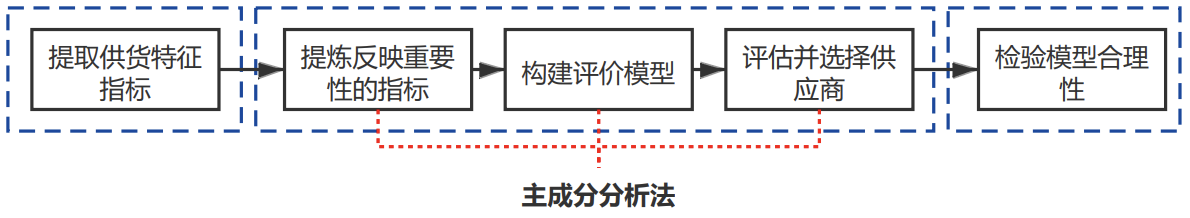
\includegraphics[width=15cm]  {问题一思路.png}}
    \caption{流程图}
\end{figure}

%----5.2 问题一模型的建立----%
\subsection{供货特征分析}
\label{5.2}

对供货特征进行分析,首先应当提取能够反映供货特征的指标。通过对过去5年的订购量和供应量数据进行分析,结合常用的数字特征、供应商评价指标\ref{ref001}和实际含义,本文归纳出了供应商供货特征的三个重要维度:供货水平,订购与供货关系,时间特征,并依据这三个重要维度,提取了共11个反映供货特征的指标。

\subsubsection{供应能力}%----供应能力----%
供应能力是从供应商自身的供应量数据出发,从整体的角度反映供应商的供货情况和供应产品的水平。供应量会受到订购情况的影响,当订购数量为0(即企业没有在此供应商处订购)时,供应数量一定为0,但并不能反映供应商的供应能力,因此在这个维度中的供应量数据都去除了订购量为0对应的部分,只考虑有订货情况下的供应情况。选取的具体指标如下:

\begin{spacing}{1.8}\textbf{(1)供应总量}\end{spacing}
供应总量反映了供应商的历史业务量,描述了在过去5年中供应量的多与少,可以反映供货的总体情况。具体计算公式为:

\begin{equation}
    SS_i=\sum_{j=1}^{24}g_{i j}\text{,}(o_{i j}\neq 0)
    %\label{速度公式}
\end{equation}

其中,$o_{i j}$和$g_{i j}$分别表示第$i$家供应商第$j$周的企业订购量和实际供货量。

\begin{spacing}{1.8}\textbf{(2)供应次数}\end{spacing}
供应商的供货次数理论上与企业的订购次数相等,描述了供应商在过去五年中为企业提供了多少次原材料,可以在一定程度上反映供应商与企业之间的合作密切关系。供货次数用$NS_i$表示,为了包含企业有订购但是供应量为0的情况,其值用订购量不为0的数据个数表示。

供应总量$SS_i$和供应次数$NS_i$之比即为供应量的平均值,表示为$AS_i=\frac{SS_i}{NS_i}$。平均供应量反映了供应商每次供应数量的平均水平,但是其可以直接用供应总量和供应次数表示,因此该指标不纳入分析体系中。

\begin{spacing}{1.8}\textbf{(3)供应量中位数}\end{spacing}
供应总量和平均数都容易受到极端值的影响。在402家供应商的数据中,有很多供应商的供应量都具有极端值,例如供应商$S201$的最大值为30977,第二大为9307,最小值仅为155,如果仅用总量或均值无法全面反映供货特征。通过因此可以通过中位数反映供货量的不受极端之影响的集中趋势,用$MeS_i$表示,其值为每家供应商$i$供货量的中位数。

\begin{spacing}{1.8}\textbf{(4)供应量方差}\end{spacing}
供应量的方差描述了供应数据的离散程度,反映了5年中供应量的波动情况,可以看出供应商供应情况的稳定性和集中性。具体计算公式为:

\begin{equation}
    VS_i=\frac{\sum_{j = 1}^{240}\left(AS_i-S_{ij}\right)^2 }{NS_i}
    %\label{速度公式}
\end{equation}

\begin{spacing}{1.8}\textbf{(5)最大供货能力}\end{spacing}
除了集中趋势外,极端值也可以在某一方面反映供货特征。最大值在一定程度上可以反映一个供应商的最大供货能力,但为了排除偶然性,这里取前两个最大值的平均值来反映最大供货能力,可表达为$MaxS_i=\frac{\text{最大供应量}+\text{第二大供应量}}{2} $。

\begin{spacing}{1.8}\textbf{(6)大供货量次数}\end{spacing}
大供货量次数指供应商单次提供大批量原材料的能力。一个供应商单次供货的数量越大,对总供货量的影响就越重要,对该周生产的影响也越大。因此,一个供应商供应大批量原材料的次数越多,也能够在一定程度上反映其对企业生产的重要性。

这里涉及如何对“大供货量”制定界限,以统计大供货量次数。由于每种原材料的数量级可能有所差异,因此将402家供应商的供应量数据按照A、B、C原材料进行分类,并去除订货量为0的数据,求出所有数据的均值$\mu $和标准差$\sigma$,以$\mu +\sigma$作为下限筛选属于大供货量的数据。通过计算得到A、B、C三种原材料的下限分别为:733、892和617,供应商大数据量总次数分别为549、173和622。分别计算出每个供应商的大供货量数据的个数,作为大供货量次数,记为$LNS_i$。

\subsubsection{订购与供货关系}%----订购与供货关系----%
订购与供货之间有着非常密切的关系,因此在分析供货特征时,与订购之间的关系是一个不可忽视的维度。这里我们重点关注供货量对订购量的满足情况,可以反映供货商供货的交付能力和可靠性。

\begin{spacing}{1.8}\textbf{(1)订购量满足率}\end{spacing}
供货满足率为供应商对企业订购量的满足程度,能够反映供货的及时性和准确性,表达为供应量与订购量之比,具体公式为:
\begin{equation}
    f_{i j}=\frac{\text{供应商i当周供应量}}{\text{供应商i当周订购量}}\times 100\%=\frac{g_{i j}}{o_{i j}}\times 100\%\text{,} \left(o_{i j}\neq 0\right)
\end{equation}

其中$f_{i j}$表示第$i$家供应商第$j$周的订购量满足率。这里分别研究供应商每周的订购量满足率的均值和方差,分别分析满足率的集中趋势和离散程度。

\ding{172} 满足率均值

满足率的均值反映了供应商交付能力的平均水平,即供应商平均每周能够满足多少采购商当周的订货量,具体表达式为:
\begin{equation}
    AF_i=\frac{\sum_{j = 1}^{240}f_{i j}}{NS_i}
\end{equation}

\ding{173} 满足率方差

满足率的方差反映了交付能力的离散情况,即过去5年供应商每周满足率的分散程度,可以体现交付能力的稳定性,具体的表达式为:
\begin{equation}
    VF_i=\frac{\sum_{j = 1}^{240}\left(f_{i j}-AF_i\right)^2 }{NS_i}
\end{equation}

\begin{spacing}{1.8}\textbf{(2)满足频数}\end{spacing}
满足率可以反映每一个供应量对订购量的满足程度,而企业的期望是使得每次的供应量都尽量满足订购量,以保障企业的正常生产,因此每家企业5年来供应量满足订购量的次数也是一个可以考虑的指标,可以反映5年中企业的准确交付情况。将这个次数称为满足频数,表达为$FC_i$,其值等于240周中供应量不小于企业订购数量的周数。

\subsubsection{时间特征}%----时间特征----%
每个供应商的供货情况都是一个跨度为240周的时间序列,因此本文将供货的时间特征也纳入需要分析的一个维度。时间序列一般由四个因素构成:周期性、趋势性、季节性和随机性。考虑到企业的订购计划是以24周为一个固定周期的,因此这里重点观察供应量的周期性,通过指标判断供应量是否也具有相应的周期特征。

该问题提供了5年共240周的订购、供货数据,我们将每一家供货商240周的供货量分10个周期进行同期考虑,求出同期的平均值,再分别对这10期的平均值求出均值、标准差与变异系数。根据这三个值,可将所有供货商供货的时间特征分为这几类:
\begin{spacing}{1.8}\textbf{(1)大量、周期性明显}\end{spacing}
这类供货商的均值较大,但变异系数较小。例如图\ref{大量、周期性明显}中的3家供货商,
\begin{figure}[H]
    \label{大量、周期性明显}
    \center{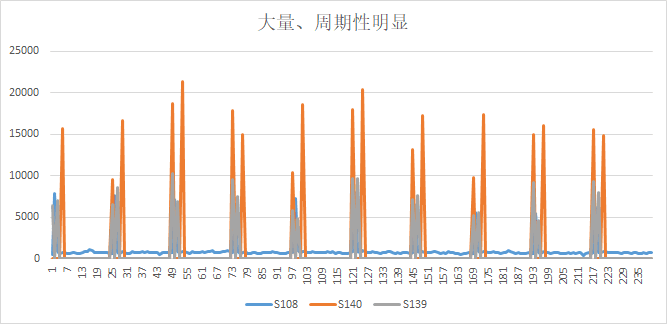
\includegraphics[width=15cm]  {大量、周期性明显.png}}
    \caption{大量、周期性明显}
\end{figure}
其均值与变异系数如表\ref{周期特征指标1}所示:
\begin{table}[h]
    \caption{周期特征指标}\label{周期特征指标1} \centering
    \centering
    \begin{tabular}{|c|c|c|c|}
    \hline
    序号 & 均值 & 变异系数 \\ \hline
    S108 & 1003.958333 & 1.203816916 \\ \hline
    S140 & 1258.529167 & 3.342889793 \\ \hline
    S139 & 632.7583333 & 3.257682447 \\ \hline
    \end{tabular}
\end{table}

\begin{spacing}{1.8}\textbf{(2)大量、周期性不明显}\end{spacing}
这类供货商的均值较大,变异系数也较大。例如图\ref{大量、周期性不明显}中的3家供货商,
\begin{figure}[H]
    \label{大量、周期性不明显}
    \center{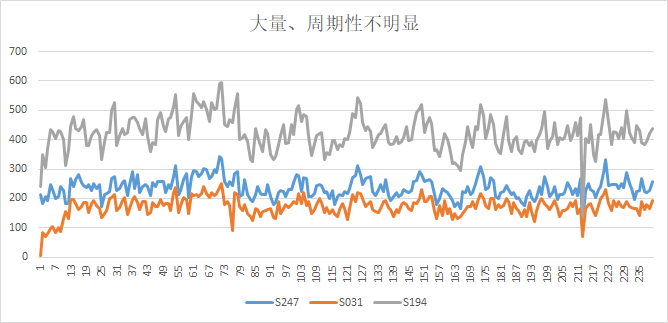
\includegraphics[width=15cm]  {大量、周期性不明显.png}}
    \caption{大量、周期性不明显}
\end{figure}
其均值与变异系数如表\ref{周期特征指标2}所示:
\begin{table}[h]
    \caption{周期特征指标}\label{周期特征指标2} \centering
    \centering
    \begin{tabular}{|c|c|c|c|}
    \hline
    序号 & 均值 & 变异系数 \\ \hline
    S247 & 236.2416667 & 0.079119526 \\ \hline
    S031 & 171.6958333 & 0.080180225 \\ \hline
    S194 & 422.3541667 & 0.082049176 \\ \hline
    \end{tabular}
\end{table}

对于小批量的订货、供货而言,其数量可能会波动。但由于其数量较少,但我们不考虑其周期性。我们主要考虑的大批量货物的周期性,其具有明显的季节特性。

%----5.3 问题一模型的建立----%
\subsection{基于主成分分析法的重要性评价模型}

\subsubsection{主成分分析法}
由于对供货特征指标的提取具有主观性,因此需要对指标进行选择和处理。一方面,\ref{5.2}一共提取了11个能够反映供货特征的指标,但是并不知道这些指标是否真正对企业生产产生明显的影响,需要对指标进行选择,找出有影响的指标来进行综合评价。另一方面,指标可能存在相互影响,需要考虑消除指标间的相互影响,提高评价的准确性。结合这一特点,本题使用主成分分析法建立评价模型具有非常好的效果。

主成分分析法是一个研究多个变量之间复杂相关性的方法,可以通过原始变量中少数几个主成分来解释多个变量间的内部结构,并使它们尽可能多地保留原始变量的信息。使用主成分分析法有明显的优势。首先,主成分之间互不相关,消除了指标间的相互影响。同时减少不必要的指标,使数据达到降维的效果,也可以减少计算量。并且,在主成分分析法的评价函数中,对各个主成分的赋权是客观的,表现为其对数据信息量的贡献率,因此可以更加客观进行评价。

主成分分析法的目标是找到原来n个变量的线性组合。主要思路为:将选取的最主要线性组合作为第一线性组合,记为$y_1$。$y_1$的方差$var(y_1)$越大,表示$y_1$包含的信息量越多。为了让$y_1$反映原来的变量尽可能多的信息,$y_1$的方差应该是所有线性组合中最大的。当第一个主成分$y_1$不足以表达n个变量的信息的时候,选取第二个主成分$y_2$,以此类推。同时,为了保证反应原来数据的指标不冗余,$y_1$已经有的信息就不应该在$y_2$中出现,则$y_1$和$y_2$应无关,$cov(y_1,y_2)=0$,一直加入新的主成分直到累计方差贡献率达到某个较高的值为止。当$var\left(y_1\right)\geq var\left(y_2\right)\geq\ldots\ \geq var(y_n)$时,可以得到协方差矩阵的特征向量$\lambda_1\ \geq\ \lambda_2\ \geq\ldots\ \geq\lambda_n$,从而转化为寻找协方差矩阵的特征值的排序。

\subsubsection{评价模型的建立与求解}
本题利用主成分分析法建立反映保障企业生产重要性的综合评价模型,用Matlab编写程序进行求解。

\noindent\textbf{步骤一:选择主成分}

\begin{spacing}{1.8}\textbf{(1)标准化}\end{spacing}
模型选择了11个指标,对每个指标的数据均进行标准化处理——将$m_{ij}$转化为${\hat{m}_{ij}}$,有:

\begin{equation}
    \widehat{m}_{i j}=\frac{m_{i j}-\mu_{j}}{s_{j}}, i=1,2, \ldots, 402, j=1,2, \ldots, 11
\end{equation}

其中,$\mu_{j}=\frac{1}{402} \sum_{i=1}^{402} m_{i j}$, 代表了第j个指标的样本平均值。

$s_{j}=\sqrt{\frac{1}{402-1} \sum_{i=1}^{402}\left(m_{i j}-\mu_{j}\right)^{2}}$ ,代表了第j个指标的样本标准差。

\begin{spacing}{1.8}\textbf{(2)协方差矩阵的计算}\end{spacing}

设协方差矩阵为$P={(p_{ij})}_{11\times11} $,对于每个$p_{ij}$,有:

\begin{equation}
    p_{ij}=\ \frac{\sum_{k=1}^{17}{\widehat{m_{ki}}\times\widehat{m_{kj}}}}{17-1}\ ,\ i=1,2,\ldots,5,\ j=1,2,\ldots,5
\end{equation}

其中,$p_{ij}$为第i个指标与第j个指标的相关系数。规定$p_{ii}=1$;$p_{ij}=p_{ji}$。

\begin{spacing}{1.8}\textbf{(3)计算协方差矩阵的特征向量和特征值,以此识别主成分}\end{spacing}
根据协方差矩阵求出特征值,并进行排序:$\lambda_1\geq\lambda_2{\geq\ldots\geq\lambda}_{11}$,对应的特征向量分别为$u_1\text{,}u_2\text{,}…\text{,}u_{11}$,其中:

\begin{equation}
    u_{i}=\left[u_{1 i}, u_{2 i}, \ldots, u_{11 i}\right]^{T}, i=1,2, \ldots, 11
\end{equation}

故对应的主成分依次为:

\begin{equation}
    \left\{\begin{array}{l}
        y_{1}=u_{11} x_{1}+u_{12} x_{2}+u_{13} x_{3}+\cdots+u_{1 n} x_{n} \\
        y_{2}=u_{21} x_{1}+u_{22} x_{2}+u_{23} x_{3}+\cdots+u_{2 n} x_{n} \\
        \ldots \\
        y_{n}=u_{n 1} x_{1}+u_{n 2} x_{2}+u_{n 3} x_{3}+\cdots+u_{n n} x_{n}
        \end{array}
    \right.
\end{equation}

\begin{spacing}{1.8}\textbf{(4)计算特征值的累计贡献率}\end{spacing}
通过计算特征值的贡献率来选择主成分。特征值$\lambda_i\ \ ,\ i=1,2,\ldots,11$ 对应的贡献率为:

\begin{equation}
    a_{i}=\frac{\lambda_{i}}{\sum_{k=1}^{11} \lambda_{k}}, \quad i=1,2, \ldots, 11
\end{equation}

其中,$\sum_{i=1}^{n}a_i $称为主成分$a_i$ 从1到n的累计贡献率,根据一个目标的累积贡献率,即可按照贡献率从大到小即可确定需要用到的主成分。

上述步骤通过Matlab进行求解,可以得到11个指标的特征值和贡献率,按特征值排序的数据结果如表\ref{tab005}所示。结合所求数据,本题采用累计贡献率大于0.93作为筛选主成分的方法代替原来的11个指标。因此,本题选取5个综合指标代替原有的11个指标,并可以算得5个综合指标的特征向量,用于建立评价模型。

\begin{table}[h]
    \caption{11个指标的特征值和贡献率}\label{tab005} \centering
    \centering
    \begin{tabular}{|c|c|c|c|}
    \hline
    序号 & 特征值 & 贡献率 & 累计贡献率 \\ \hline
    1 & 5.7489 & 52.2631 & 52.2631 \\ \hline
    2 & 2.0048 & 18.2252 & 70.4882 \\ \hline
    3 & 1.5296 & 13.9055 & 84.3937 \\ \hline
    4 & 0.7441 & 6.7642 & 91.1579 \\ \hline
    5 & 0.3465 & 3.1504 & \textbf{94.3083} \\ \hline
    6 & 0.2914 & 2.6487 & 96.9570 \\ \hline
    7 & 0.1772 & 1.6113 & 98.5683 \\ \hline
    8 & 0.1374 & 1.2493 & 99.8176 \\ \hline
    9 & 0.0136 & 0.1236 & 99.9412 \\ \hline
    10 & 0.0065 & 0.0588 & 100.0000 \\ \hline
    11 & 0.0000 & 0.0000 & 100.0000 \\ \hline
    \end{tabular}
\end{table}

\noindent\textbf{步骤二:建立主成分的综合评价模型}

对步骤一中选择的主成分进行综合分析,并按照得分高低降序排序,即可建立评价函数,一般形式为:

\begin{equation}
    Z=\sum_{j=1}^{q} a_{j} \times y_{j}
\end{equation}

其中,Z为某评价单位的主成分分析得分;q为第四步中确定的主成分个数。

步骤一的求解得到了5个主成分,并求出了对应的特征向量。分别以这5个主成分的贡献率为权重,建立本题的综合评价模型:

\begin{equation}
    Z=0.5226y_1+0.1823y_2+0.1391y_3+0.0676y_4+0.03150y_5
    \label{评价模型}
\end{equation}

其中,$y_{i}=u_{i 1} x_{1}+u_{i 2} x_{2}+u_{i 3} x_{3}+\cdots+u_{i 11} x_{11}$,$x_j$表示第$j$个指标的值,$u_{i j}$为第$i$个主成分的特征向量的元素。

\subsubsection{问题一的解答与分析}

将\ref{5.2}中计算得到的402家供应商11个指标的数据带入\ref{评价模型}求得的评价模型,即可得到每个供应商的综合评价得分,得分越高表示其重要性越高,按得分对供应商进行排序,即可得到前50家对保障企业生产最重要的供应商,结果如下表\ref{第一问结果}所示:

\begin{table}[h]
    \caption{第一问求解结果}\label{第一问结果} \centering
    \centering
    \begin{tabular}{|c|c|c|c|c|c|c|c|c|}
    \hline
    \textbf{排名} & \textbf{供应商} & \textbf{得分} & \textbf{排名} & \textbf{供应商} & \textbf{得分} & \textbf{排名} & \textbf{供应商} & \textbf{得分}\\\hline
    1 & S140 & 12.3397 & 19 & S268 & 2.6048 & 37 & S080 & 1.0770 \\ \hline
    2 & S229 & 6.5265 & 20 & S131 & 2.5634 & 38 & S346 & 1.0732 \\ \hline
    3 & S151 & 6.2086 & 21 & S395 & 2.3211 & 39 & S218 & 1.0656 \\ \hline
    4 & S361 & 6.0497 & 22 & S126 & 2.2736 & 40 & S114 & 1.0416 \\ \hline
    5 & S201 & 5.9820 & 23 & S194 & 2.0968 & 41 & S294 & 1.0373 \\ \hline
    6 & S139 & 5.8409 & 24 & S143 & 2.0031 & 42 & S244 & 1.0227 \\ \hline
    7 & S108 & 5.6581 & 25 & S352 & 1.9455 & 43 & S007 & 0.9467 \\ \hline
    8 & S348 & 5.5682 & 26 & S037 & 1.7591 & 44 & S266 & 0.9296 \\ \hline
    9 & S374 & 3.9552 & 27 & S338 & 1.6703 & 45 & S291 & 0.9020 \\ \hline
    10 & S307 & 3.9049 & 28 & S284 & 1.5987 & 46 & S123 & 0.8536 \\ \hline
    11 & S282 & 3.8385 & 29 & S247 & 1.5412 & 47 & S150 & 0.8044 \\ \hline
    12 & S330 & 3.1889 & 30 & S365 & 1.4055 & 48 & S003 & 0.7733 \\ \hline
    13 & S340 & 3.1351 & 31 & S055 & 1.3697 & 49 & S314 & 0.7420 \\ \hline
    14 & S275 & 3.1010 & 32 & S031 & 1.3386 & 50 & S098 & 0.7192 \\ \hline
    15 & S356 & 3.0669 & 33 & S364 & 1.3036 &  &  &  \\ \hline
    16 & S308 & 3.0528 & 34 & S040 & 1.2695 &  &  &  \\ \hline
    17 & S329 & 3.0483 & 35 & S086 & 1.2109 &  &  &  \\ \hline
    18 & S306 & 2.6836 & 36 & S367 & 1.1938 &  &  &  \\ \hline
    \end{tabular}
\end{table}

通过对前50家供应商相关指标的分析,来观察结果和模型的合理性。

(1)从供货总量来看,402家中供货总量大于10万的17家产业全部被筛选了出来,供货量大印证了企业对于该供应商的依赖程度高。

(2)原材料满足率平均值上,绝大多数企业的平均值达到了0.99及以上,同时,绝大多数企业在240周内满足订单的次数大于150次,代表企业的订货需求在这些供应商中容易被满足。

(3)除了含有特殊周期性规律的201号供应商之外,企业对各供应商的订货次数都较多,50家企业中有36家订货次数全满,为240次。

(4)特殊的201号供应商也成功筛选出来,它总订货量很大,虽然订货次数较少,但是完成了很多大供应量的订购,说明企业对201号供应商也较为重视。

总体上,主成分分析法筛选出的50家供应商,从指标的角度可以得出企业对他们重视程度高,依赖性强的特点,从而侧面证明了选取的指标具有代表性和主成分分析的合理性。




% %----5.4 问题一的求解---%
% \subsection{结果分析}
% \textcolor{red}{把实际问题归结为一定的数学模型后,就要利用数学模型求解所提出的实际问题了。一般需要借助计算机软件进行求解,例如常用的软件有 Matlab, Spss, Lingo, Excel, Stata, Python 等。求解完成后,得到的求解结果应该规范准确并且醒目,若求解结果过长,最好编入附录里。(注意:如果使用智能优化算法或者数值计算方法求解的话,需要简要阐明算法的计算步骤)}
% 注意要对结果进行适当的分析,说明其合理性。

% 例一:

% 根据我们编写的迭代算法,即可获得三位玩家选择的路线,如右图所示,可以看出,一位玩家沿上边界和右边界到达终点,一位玩家沿左边界和下边界到达终点,还有一位玩家从地图中部到达终点;根据题意可知,该路线是比较合理的,因为若 有多个玩家选择同一条路线,则他们资源的消耗量增大,挖矿获得的基础收益降低,同时若要前往村庄补给物资,则购买价格也会增加;所以玩家应选择尽量不同的路线,这与我们得到的路线是相符的。

% 例二:

% 我们使用蒙特卡洛方法对该模型进行仿真,即对于第四问的情况,使用 C++中的rand()函数随机生成天气的情况,但此处各种天气的出现频率必须满足“较少出现沙暴” 的要求,因此我们限定沙暴天气最多出现3天,一次仿真后得到:参与者到达终点时剩余资金数为11245元,参与者在起点购买的食品190箱,水171箱,可以发现该仿真结果与使用在第一关、第二关天气数据上稍作修改得到的结果类似,因此模型较为合理。


%-------------------- 问题二模型的建立与求解 --------------------%
\section{问题二:供应商选择、订购方案、转运方案决策模型}
\subsection{问题分析}
订购方案和转运方案都需要给出每周的具体方案,依据假设\ref{供应能力假设},结合实际情况,本题认为每个供应商或转运商每周会有不同的供应能力或转运损耗率,因此每周的订购方案和转运方案也会不同。由于订购和转运方案都以24周为制定周期,因此在考虑供货商的供货量和转运商的损耗率时,都也以24周为一个周期,考虑每一周的具体情况。

由于题目给出了过去5年240周的历史数据,因此本文将240周数据以24周为跨度其拆分成10个周期,对10个周期中每一周的数据进行同期分析,通过历史数据来确定供货情况和损耗率的情况,为订购方案和转运方案提供依据。

%----6.2 问题二模型的建立----%
\subsection{基于0-1整数规划的供应商选择模型}
\subsubsection{模型的建立}
\label{供应量的确定}

\noindent\textbf{(1)每周供应量的确定}

在对订购方案进行规划时,需要考虑供应商每周的供应量,以保证原材料能够满足计划的生产。每家供应商每周的供应量用$c_{i j}$表示,它是一个随机变量,但为了能够规划出一个最优方案,本题结合问题一中的指标,通过每家供应商24周中每周的10个历史数据来确定一个预期供应量,提供两种计算方法:

(1)每家供应商每周都以当周的最大供应能力提供原材料,这是一个相对理想的情况,现实中供应商难以都按照最大供应能力供货。根据问题一中最大供应能力这一指标的计算方法,可以计算得到$c_{i j}$。

(2)每家供应商每周以平均供应水平提供原材料,这是一个平均情况。根据问题一中平均供应量这一指标的计算方法,可以计算得到$c_{i j}$。

对于转运商的损耗率,可以同样用这两种方法求出转运商$i$在第$j$周的预期损耗率$dis_{ij}$

\noindent\textbf{(2)建立0-1整数规划模型}

根据2.2,步骤一只涉及供应商的选择与否,因此通过建立0-1整数规划求解。用0-1变量表示本次订购方案是否选择某一家供应商,表示为:

\begin{equation}
    x_i=
    \begin{cases}
        1\text{,选择第i家供应商}\\
        0\text{,不选择第i家供应商}
    \end{cases}
\end{equation}

目标函数为最小化选择的供应商的数量,因此可以直接用0-1变量的和表示,表达为:

\begin{equation}
    \min \sum_{i = 1}^{|S|}  x_i
\end{equation}

约束条件主要有两个方面,首先是要求选择的供应商可能满足生产的需求,其次是尽量保持维持两周生产的库存。可能满足需求是一个比较理想的情况,因此考虑用第一种方法计算$c_{i j}$,得到的方案也是一个比较理想的方案。首先,要满足生产的需求,就要尽可能使订购原材料能够生产的产品数量等于生产计划量2.82万立方米。但是,通过对$c_{i j}$的分析可以发现,不一定每周都能够有足够的供应量支持生产。因此可以允许某一周使用库存来弥补当周不足的供应量。添加一个松弛变量$s_k$来表示第k周使用库存的数量,添加一个参数$S_{max}$表示一周允许使用的库存数量的上限,则$s_k\leq S_{max} $。因此每周的生产量为原材料供应量(要基于本供应商原材料与产品转换比例${\alpha_i }$进行换算)和使用的库存量之和。但由于每周仍要尽可能维持两周的库存,因此应当使前$k$周订购量的总和满足前$k$周的总生产需求,以提前订购需要使用的库存,因此该约束条件可以表示成:

\begin{equation}
        \sum_{j = 1}^{k}  \sum_{i = 1}^{|S|} \frac{c_{i j}}{\alpha_i}x_i+s_k=2.82\times k
        \label{满足生产约束条件}
\end{equation}

其中$k=1,2,3...,24$,$|S|$表示本次制定方案可选择的供应商的数量。

综上所述,选择供应商的模型建立如下:
\begin{equation}
    \min \sum_{i = i}^{|S|} x_i 
\end{equation}

\begin{equation}
    \begin{cases}
        \sum_{j = 1}^{k}  \sum_{i = 1}^{|S|} \frac{c_{i j}}{\alpha_i}x_i+s_k=2.82\times k\text{,}k=1,2,3...,24\\
        s_k\leq S_{m a x}\text{,}k=1,2,...,24
    \end{cases}
\end{equation}

\subsubsection{模型的求解与分析}
由于该模型是一个整数线性规划模型,可以通过分支定界等方法进行求解。分支定界法的基本思想是,对于一个含有整数约束的规划问题,先求其松弛问题的解作为下界。若解不满足整数约束,则进行分支;若满足,则作为上界;一直递归,直到上界等于下界。

本文通过Python调用求解器——Gurobi求解整数线性规划模型。Gurobi求解器作为行业顶尖的求解器,在求解整数规划方面有很好的效果。最终求解得到供应商的数量为16家,即至少需要16家供应商,才可能满足生产。具体的16家供应商为:S108,S131,S139,S140,S151,S201,S229,S275,S307,S308,S329,S330,S340,S348,S361,S395。

将这16家供应商与问题一中得到的最重要前50家供应商进行对比可以发现,这16家供应商都位于问题一中保障企业生产重要性的前22家。其中最重要的前8名供应商都被选择,对比结果如下表所示。因此本题的结果与问题一中的评价结果是相符的,一方面说明了这16家供应商选择的合理性,也可以进一步体现出问题一的评价模型的合理性。

\begin{table}[h]
    \caption{16家供应商的问题一排序}\label{tab005} \centering
    \centering
    \begin{tabular}{|c|c|c|c|c|c|}
    \hline
    排名 & 供应商 & 得分 & 排名 & 供应商 & 得分 \\ \hline
        1 & \textcolor{red}{\textbf{140}} & 12.3397 & 12 & \textcolor{red}{\textbf{330}} & 3.1889 \\ \hline
        2 & \textcolor{red}{\textbf{229}} & 6.5265 & 13 & \textcolor{red}{\textbf{340}} & 3.1351 \\ \hline
        3 & \textcolor{red}{\textbf{151}} & 6.2086 & 14 & \textcolor{red}{\textbf{275}} & 3.1010 \\ \hline
        4 & \textcolor{red}{\textbf{361}} & 6.0497 & 15 & 356 & 3.0669 \\ \hline
        5 & \textcolor{red}{\textbf{201}} & 5.9820 & 16 & \textcolor{red}{\textbf{308}} & 3.0528 \\ \hline
        6 & \textcolor{red}{\textbf{139}}& 5.8409 & 17 & \textcolor{red}{\textbf{329}} & 3.0483 \\ \hline
        7 & \textcolor{red}{\textbf{108}} & 5.6581 & 18 & 306 & 2.6836 \\ \hline
        8 & \textcolor{red}{\textbf{348}} & 5.5682 & 19 & 268 & 2.6048 \\ \hline
        9 & 374 & 3.9552 & 20 & \textcolor{red}{131} & 2.5634 \\ \hline
        10 & \textcolor{red}{\textbf{307}} & 3.9049 & 21 & \textcolor{red}{\textbf{395}} & 2.3211 \\ \hline
        11 & 282 & 3.8385 &  &  &  \\ \hline
    \end{tabular}
\end{table}

%----6.3 问题二的求解---%
\subsection{基于整数规划的采购方案决策模型}
\subsubsection{模型分析}
对于上面这确定的16家供应商,制定最经济的未来24周每周的订购计划,根据2.2,考虑建立整数规划模型求解。由于这一步只考虑订购计划,因此将这里的``经济''理解为采购成本最小,因此目标函数为订购总成本最小化。约束条件仍为应满足生产的计划,同时不能超过供应商的可提供的原材料数量。由于这16家企业是在理想情况下得到的,因此这里参考的供应量也应使用最大供应能力。

\subsubsection{模型的建立和求解}

设整数变量$x_{ij}$表示第i家供应商第j周的订购量。目标函数为订购成本最小化,由于题目没有给出具体的价格,只说明了A、B、C三种材料的成本比例关系,因此这里将C的采购成本设定为1。因此目标函数可表达为:

\begin{equation}
    \min \sum_{i = 1}^{|S|} \sum_{j = 1}^{24} p_i x_{ij}
\end{equation}

其中,$p_i$表示第i家供应商提供的原材料对应的单位成本。

满足企业生产这一约束条件与约束条件(\ref{满足生产约束条件})一致,在每周完成2.82万立方米生产的条件下,允许使用库存满足某一周的生产。并且当周在某一家供应商的订购量不能超过供应商的最大供应量$c_{i j}$。因此增加约束条件:

\begin{equation}
    x_{ij}\leq c_{ij}
\end{equation}

同时,还要考虑到每周的订购总量不能超过8家转运商每周的最大转运量,用$t_{\mathrm{max}}|T|$。其中$t_{\mathrm{max}}$表示单家转运商的一周最大转运量6000,$|T|$表示转运商的数量,约束条件为:

\begin{equation}
    \sum\limits_{i = 1}^{|S|} x_{ij} \leq t_{\mathrm{max}}|T|
\end{equation}

综上所属,采购方案的决策模型如下:

\begin{equation}
    \min \sum_{i = 1}^{|S|} \sum_{j = 1}^{24} p_i x_{ij}
\end{equation}

\begin{equation}
    \begin{cases}
        \sum_{j = 1}^{k}  \sum_{i = 1}^{|S|} \frac{x_{i j}}{\alpha_i}+S_k=2.82\times k\text{,}k=1,2,3...,24\\
        S_k\leq S_{m a x}\text{,}k=1,2,...,24\\
        x_{ij}\leq c_{ij}\\
        \sum\limits_{i = 1}^{|S|} x_{ij} \leq t_{\mathrm{max}}|T|
    \end{cases}
\end{equation}

同样对模型进行求解,得到16家供应商的24周订购方案,具体方案见附件A,得到最低订购成本为$488652.8a$,其中$a$为产品C的订购单价。


%----6.3 问题二的求解---%
\subsection{基于指派问题思想的订购方案决策模型}
\subsubsection{模型分析}
步骤三基于这个确定的24周的订购方案,来制定损耗最少的转运方案。根据题意,这里的损耗指的是损耗量,为转运量与损耗率的乘积。首先,由于每周的订购方案是确定的,并且每周的供货要全部转运完毕,因此以周为单位对转运方案进行规划。由于一家供应商的原材料尽量由一家转运商转运,因此在供应量不超出一家转运商的最大转运量时,一家供应商只选择一家转运商转运,并且这个数量是已知的。选择不同的转运商,会面临不同的损耗,需要找到一种选择方案使得总损耗最小。这一选择方法符合指派问题的思想,因此这一小问基于指派问题的基本思想建立模型。

\subsubsection{模型的建立和求解}
\noindent\textbf{(1)指派问题}

基础的指派问题通常解决这样一类问题:有一定数量的任务和的员工,需要保证每个任务都有人完成,每个员工都完成一项任务。每个员工都可以完成任意任务,但是所需要的成本不同。需要寻找一种指派方案,使得总的成本最小。

指派问题的基础模型为:
\begin{equation}
    min z=\sum_{i = 1}^{n} \sum_{j = 1}^{n}  c_{ij}x_{ij}
    \label{指派问题目标函数}
\end{equation}

\begin{equation}
    \begin{cases}
        \sum_{i = 1}^{n} x_{ij}=1\text{,} j=1,...,n\\
        \sum_{j = 1}^{n} x_{ij}=1\text{,} i=1,...,n\\
    \end{cases}
    \label{指派问题约束条件}
\end{equation}

在这一问题中,转运商就是需要完成任务的员工,任务为对供应商提供的货物进行转运。在这一思想的基础上面,本问题建立0-1整数规划进行求解。

\noindent\textbf{(2)订购方案决策模型的建立}

本题的目标函数为总损耗最小,对于指派问题中的目标函数(\ref{指派问题目标函数}),$c_{ij}$表示第i家供应商的货物由第j家转运商进行转运的损耗。由\ref{供应量的分析}中计算供应量的两种情况,这里对转运方案的规划应当是基于一般情况下的最优解,因此计算损耗率$dis_{ij}$的均值,得到每家转运商的预期损耗率。由于每周每家供应商对应的转运量$trans_i$,是确定的,因此$c_{ij}$就为$dis_{ij}\times trans_i$。每个供应商对转运商的选择结果用$u_{ij}$表示。因此目标函数表示为:

\begin{equation}
    min \sum_{i = 1}^{|S|}  dis_{ij}\times trans_i \times u_{ij}
\end{equation}

但本题还面临转运商转运能力的约束。当一家供应商的供货量超过一家转运商的转运能力$t_{\mathrm{max}}$时,就需要分多家转运商进行转运。但是由于仍要满足转运商数量尽可能少,因此可以考虑将大于转运能力的一批原材料以6000为界限拆分成多批,用多个0-1变量$u_{ij}$来表示这一批原材料选择的转运上的情况。这样就仍可以用此模型进行解决。这里只需要满足每个供应商选择一家转运商,因此约束条件(\ref{指派问题约束条件})在此处为:

\begin{equation}
    \sum_{j = 1}^{|T|} u_{ij}=1\text{,} i=1,...,|S|
\end{equation}

这里还需要加上对转运商每周转运能力的限制:

\begin{equation}
    \sum_{i = 1}^{|S|} u_{ij}\leq t_{\mathrm{max}}\text{,} j=1,...,|T|
\end{equation}

综上所述,订购方案决策模型表示如下:
\begin{equation}
    min \sum_{i = 1}^{|S|}  dis_{ij}\times trans_i \times u_{ij}
\end{equation}

\begin{equation}
    \begin{cases}
        \sum_{j = 1}^{|T|} u_{ij}=1\text{,} i=1,...,|S|\\
        \sum_{i = 1}^{|S|} u_{ij}\leq t_{\mathrm{max}}\text{,} j=1,...,|T|\\
    \end{cases}
\end{equation}

\noindent\textbf{(3)模型的求解}

基于此0-1整数规划问题,分别对24周进行求解,可以得到本题订购方案对应的每周损耗最小的转运方案。具体方案见附件B,得到每周的最低损耗情况如下表:

\begin{table}[h]
    \caption{第二问转运方案损耗结果}\label{tab005} \centering
    \centering
    \begin{tabular}{|c|c|c|c|c|c|}
    \hline
    & \textbf{损耗量} &  & \textbf{损耗量} &  & \textbf{损耗量} \\ \hline
        第1周 & 958.8230 & 第10周 & 186.3398 & 第19周 & 407.4986 \\ \hline
        第2周 & 203.1473 & 第11周 & 327.7321 & 第20周 & 183.2760 \\ \hline
        第3周 & 267.4422 & 第12周 & 394.2897 & 第21周 & 76.6668 \\ \hline
        第4周 & 101.1152 & 第13周 & 439.5795 & 第22周 & 76.9400 \\ \hline
        第5周 & 608.3642 & 第14周 & 214.6537 & 第23周 & 278.0339 \\ \hline
        第6周 & 283.4216 & 第15周 & 162.0531 & 第24周 & 199.0707 \\ \hline
        第7周 & 95.5070 & 第16周 & 97.4596 &  &  \\ \hline
        第8周 & 99.8850 & 第17周 & 225.9578 &  &  \\ \hline
        第9周 & 131.8195 & 第18周 & 247.2663 & \textbf{损耗总量} & \textbf{2749.5249} \\ \hline
    \end{tabular}
\end{table}

\subsection{方案评价}
\subsubsection{订购方案评价}

通过与历史订购数据的对比分析来评价本题的订购方案。第二问中本文选取了16个重要原材料供应商,采用的订购策略在24周最经济的条件下最终计算得订购总花费为$488652.8a$,计算求得前五年以24周划分的周期的每周期平均订购总花费为$484048.4a$,与我们订购方法的结果相比,节约了$4604.4a$,但由于本次设计的订购方案使企业保持每周库存量均大于等于两周生产所需的原材料数量,而原始数据则没有这个条件,最终我们仅多出了总价的0.94\%,误差较小,所以此模型满足了最经济的原材料订购方案的要求。


\subsubsection{转运方案评价}
\noindent\textbf{(1)结果合理性分析}

从第三问的运输方案结果来看,在402家供应商的基础上,为了减少转运损耗量,最优的解会首先让转运损耗量的均值较小的转运商(如T2,T3,T6)尽可能达到转运的最大荷载能力(6000立方米/周)。 所以在供应量较大的主要供应商达到极限供应量之后,剩余不足6000立方米的部分由其余的供应量较小的供应商提供少量原材料,从而出现了如附件B中第七周的T2转运商(表中AY列)的情况——一些供应商提供了少量原材料使最终运输量达到6000立方米/周。这个结论解释了近五年402家供应商的数据中出现非常多单周1立方米的原因,符合题意,从而侧面印证了我们建立的模型及求解结果对于模型的适配性良好。

\noindent\textbf{(2)转运方案对比分析}

规划转运方案一个非常重要的因素就是对每个供应商对应转运商数量的限制,直接影响了转运的选择。本题充分考虑了一家转运商的材料尽量由一家转运商转运这一条件。这里通过对本题的方案与不考虑这一约束条件的方案进行对比,来对转运方案的实施效果进行评估。

不考虑选择的转运商数量时,只需要用整数规划模型即可求出最优解。将决策变量$v_{ij}$定为第$i$家供应商由第$j$家转运商转运的数量,目标函数为损耗率$dis_{ij}$与$v_{ij}$的乘积。约束条件只有对转运商最大转运能力的限制,建立模型如下。对模型进行求解得到一个不考虑一批原材料尽可能选择同一家转运商的转运方案,将损耗率的结果与本题求解得到的结果进行对比,如下表所示。

\begin{table}[h]
    \caption{转运方案损耗结果对比}\label{tab005} \centering
    \centering
    \begin{tabular}{|c|c|c|c|c|c|c|c|}
    \hline
    & \textbf{本题损耗量} & \textbf{对比损耗量} & \textbf{差值} &  & \textbf{本题损耗量} & \textbf{对比损耗量} & \textbf{差值} \\ \hline
    1 & 958.8230 & 954.2090 & 4.6140 & 13 & 439.5795  & 438.4051  & 1.1744  \\ \hline
        2 & 203.1473 & 203.1473 & 0.0000 & 14 & 214.6537  & 214.6488  & 0.0049  \\ \hline
        3 & 267.4422 & 267.1253 & 0.3169 & 15 & 162.0531  & 161.7757  & 0.2774  \\ \hline
        4 & 101.1152 & 101.1103 & 0.0049 & 16 & 97.4596  & 97.3561  & 0.1035  \\ \hline
        5 & 608.3642 & 607.2530 & 1.1111 & 17 & 225.9578  & 225.9234  & 0.0344  \\ \hline
        6 & 283.4216 & 283.1951 & 0.2265 & 18 & 247.2663  & 245.8545  & 1.4118  \\ \hline
        7 & 95.5070 & 95.5070 & 0.0000 & 19 & 407.4986  & 407.4718  & 0.0268  \\ \hline
        8 & 99.8850 & 99.8776 & 0.0074 & 20 & 183.2760  & 183.2465  & 0.0295  \\ \hline
        9 & 131.8195 & 131.0733 & 0.7461 & 21 & 76.6668  & 76.1197  & 0.5472  \\ \hline
        10 & 186.3398 & 186.3300 & 0.0098 & 22 & 76.9400  & 76.5259  & 0.4141  \\ \hline
        11 & 327.7321 & 327.7321 & 0.0000 & 23 & 278.0339  & 278.0154  & 0.0185  \\ \hline
        12 & 394.2897 & 393.5416 & 0.7480 & 24 & 199.0707  & 198.8153  & 0.2554  \\ \hline
         &  &  &  & \textbf{总量} & \textbf{6266.3424}  & \textbf{6254.2598}  & \textbf{12.0826}  \\ \hline
    \end{tabular}
\end{table}

在去除这一约束条件后,对供应商的选择情况更加丰富,结果会更优。但是本题在考虑了这一约束后的24周损耗率总量只比原来减少了12.0826立方米,减少了0.2\%,因此本题的转运方案效果相对是较好的。

%-------------------- 问题三模型的建立与求解 --------------------%
\section{问题三:基于多目标规划的订购和转运决策模型}

%----7.1 问题分析---%
\subsection{模型分析}
在第二问中,我们考虑的成本主要是订货成本。若C类原材料的价格为单位价格,则A、B、C三类原材料的价格分别是1.2, 1.1, 1;又由于生产1立方米的产品分别需要0.6, 0.66, 0.72立方米的原材料,因此用A、B、C来生产每立方米产品所需要的花费分别为0.72, 0.726, 0.72,大致相等。但是,若该企业选择订购C材料,则订购量比订购A、B大,较大的定购量会带来较大的转运和仓储成本。

因此,对于订购方案规划,本问在第二问的规划问题的基础上,引入了另一目标,即尽量多地采购A材料、尽量少地采购C材料,通过多目标规划的方法解决该问题。对于转运方案规划,模型和求解与上一问相同。因此,问题三本文将重点讨论订购方案的规划。

另外,这一问将在所有402家供应商中考虑订购与转运方案。

\subsection{模型建立}

根据以上分析,我们建立了以下的多目标规划模型:
\begin{gather}
    \min \{f_1, f_2, f_3\}\\
    f_1 = \sum\limits_{i=1}^{|S|}\sum\limits_{j=1}^{|W|}p_i x_{ij}\\
    f_2 = -\sum\limits_{i \in S_A}\sum\limits_{j=1}^{|W|}x_{ij}\\
    f_3 = \sum\limits_{i \in S_C}\sum\limits_{j=1}^{|W|}x_{ij}
\end{gather}

\begin{equation}
    \mathrm{s.t.}
    \begin{cases}
        \sum\limits_{j = 1}^{k}  \sum\limits_{i = 1}^{|S|} \frac{x_{ij}}{\alpha_i}+s_k=kp_d, k=1,2,\cdots,|W|\\
        s_k\leq s_{\mathrm{max}}, k=1,2,\cdots,|W|\\
        x_{ij}\leq c_{ij}, i,j = 1,2,\cdots,|S|\\
        \sum\limits_{i = 1}^{|S|} x_{ij} \leq t_{\mathrm{max}}|T|, j = 1,2,\cdots,|W|\\
        x_{ij} \in \mathbb{N}
    \end{cases}
\end{equation}
其中$f_1$为订购的原材料总价格函数,$f_2$为原材料A的订购量函数,$f_3$为原材料C的订购量函数,模型以这三者作为最小化目标。约束$\sum\limits_{j = 1}^{k}  \sum\limits_{i = 1}^{|S|} \frac{x_{ij}}{\alpha_i}+s_k=kp_d$保证了每周在使用$s_k$库存的基础上能够有充足的原材料供应,约束$s_k\leq s_{\mathrm{max}}$限制了每周能够使用的最大库存,约束$x_{ij}\leq c_{ij}$根据供应商的供货能力限制了其每周能够供给材料的最大值,约束$\sum\limits_{i = 1}^{|S|} x_{ij} \leq t_{\mathrm{max}}|T|$则保证了所订货物量不超过转运商的能力。

\subsection{模型求解}

对该模型进行求解时,我们采用加权法将多目标规划问题转化为单目标规划问题,即将目标函数转化为:
\begin{equation}
    \min F = w_1f_1 + w_2f_2 + w_3f_3
\end{equation}
转化完成后,该模型便是一个混合整数线性规划模型,可以用分支定界等方法进行求解。在数值实验中,我们使用Python调用Gurobi求解器,设置模型参数$s_{\mathrm{max}} = 0, w_1 = 1, w_2 = w_3 = 0.2$,$c_{ij}$取每24周供货量的平均值以反映供货商的供货能力,其他参数根据题意即可确定。

\subsection{结果分析}

根据求解结果,我们得到该厂家未来24周需要订购的各种原材料的总量与总价如表\ref{Q3_O_C-A}。

\begin{table}[h]
    \caption{订购总量}\label{Q3_O_C-A} \centering
    \centering
    \begin{tabular}{|p{2.0cm}<{\centering}|p{9.0cm}<{\centering}|}
    \hline
    \textbf{种类} & \textbf{数量} \\ \hline
    A           & 188021         \\ \hline
    B           & 151862         \\ \hline
    C           & 96004          \\ \hline
    总量        & 435887 \\ \hline
    总价         & 488677.4          \\ \hline
    \end{tabular}
\end{table}

然后,在订购方案的基础上通过问题二中的转运方案规划的模型进行求解,得到问题三的转运方案。详细结果见附件A、B。

在对结果的正确性进行分析时,我们考虑实际供应链中运输和储存的单位费用,记为$w_f$。生产总成本$F_c$为订购、运输和储存成本的总和,即:
\begin{equation}
    F_c = f_1 + w_f(f_2 + f_3 + f_4)
\end{equation}
$f_1, f_2, f_3$的含义与7.2中相同,$f_4 = \sum\limits_{i \in S_B}\sum\limits_{j=1}^{|W|}x_{ij}$。该企业的生产能力大致稳定,于是:
\begin{equation}
    \frac{f_2}{\alpha_A} + \frac{f_3}{\alpha_B} + \frac{f_4}{\alpha_C} \approx |W|p_d
\end{equation}
因此,若以$\min F_c$为目标,由于运输和储存成本的存在,最优解也会尽量多地采购A材料、尽量少地采购C材料。假设运输和储存的单位成本$w_f = 0.2$,则以该目标求解该规划问题得到的结果如\ref{Q3_O_A+B+C}。

\begin{table}[h]
    \caption{订购总量}\label{Q3_O_A+B+C} \centering
    \centering
    \begin{tabular}{|p{2.0cm}<{\centering}|p{9.0cm}<{\centering}|}
    \hline
    \textbf{种类} & \textbf{数量} \\ \hline
    A           & 188019         \\ \hline
    B           & 151858         \\ \hline
    C           & 96010          \\ \hline
    总量        & 435887 \\ \hline
    总价         & 488676.6          \\ \hline
    \end{tabular}
\end{table}

该解与上面的解差距很小,因此我们的结果是可靠的。

\subsection{方案评价}

我们通过对比单目标规划与多目标规划的结果来对订购方案进行评价。若仅仅以订购花费的总价格作为目标函数,得到A、B、C三类原材料的订购总量和总价如\ref{Q3_O_0}。

\begin{table}[h]
    \caption{订购总量}\label{Q3_O_0} \centering
    \centering
    \begin{tabular}{|p{2.0cm}<{\centering}|p{9.0cm}<{\centering}|}
    \hline
    \textbf{种类} & \textbf{数量} \\ \hline
    A           & 188013         \\ \hline
    B           & 99060         \\ \hline
    C           & 153615          \\ \hline
    总量        & 440688 \\ \hline
    总价         & 488196.6          \\ \hline
    \end{tabular}
\end{table}

可以看出,与加入转运和储存成本规划之前相比,原材料总价仅仅多了480元左右,但总量少了约4800立方米,可以节省下很多转运与储存成本。

%-------------------- 问题四模型的建立与求解 --------------------%
\subsection{企业订购原则}


\section{问题四:提高产能的决策模型}

%----8.1 问题分析---%
\subsection{问题分析}

本问要在已有的供应商和转运商条件下增加产能,产能增加的量受供应商和转运商的情况约束:如果供应商不能提供充足的货源、转运商没有足够的能力把货源转运到企业,产能就不能得到有效的提升。另外,产能应该是一个稳定的值,即每个周的产能应该恒定。如果某几周产能较大,某几周产能又较小,企业的设备就会闲置,这不符合生产与运营管理的理念。

因此,本问将以最大化产能为目标、以供应商和转运商的情况为约束建立规划模型。

%----8.2 问题四模型的建立----%
\subsection{模型建立}
根据以上分析,我们建立了以下的规划模型:
\begin{gather}
    \max P_{max}
\end{gather}

\begin{equation}
    \mathrm{s.t.}
    \begin{cases}
        \sum\limits_{j = 1}^{k}  \sum\limits_{i = 1}^{|S|} \frac{x_{ij}}{\alpha_i}+s_k=kP_{max}, k=1,2,\cdots,|W|\\
        s_k\leq s_{\mathrm{max}}, k=1,2,\cdots,|W|\\
        x_{ij}\leq c_{ij}, i,j = 1,2,\cdots,|S|\\
        \sum\limits_{i = 1}^{|S|} x_{ij} \leq t_{\mathrm{max}}|T|, j = 1,2,\cdots,|W|
        x_{ij} \in \mathbb{N}
    \end{cases}
\end{equation}
模型以产能$P_{max}$作为最大化目标。约束$\sum\limits_{j = 1}^{k}  \sum\limits_{i = 1}^{|S|} \frac{x_{ij}}{\alpha_i}+s_k=kP_{max}$保证了每周在使用$s_k$库存的基础上能够有充足的原材料供应,约束$s_k\leq s_{\mathrm{max}}$限制了每周能够使用的最大库存,约束$x_{ij}\leq c{ij}$根据供应商的供货能力限制了其每周能够供给材料的最大值,约束$\sum\limits_{i = 1}^{|S|} x_{ij} \leq t_{\mathrm{max}}|T|$则保证了所订货物量不超过转运商的能力。

%----8.3 问题四的求解---%
\subsection{模型求解}%----5.4.2 模型的求解---%
该模型同样也是一个整数线性规划的模型,可以用分支定界等方法求出精确解。然后,在订购方案的基础上通过问题二中的转运方案规划的模型进行求解,得到问题三的转运方案。详细结果见附件A、B。

\subsection{结果分析}

通过模型的建立与求解,得到最终产能可以提升至31013立方米每周,同时规划出了最终的订购与转运方案。根据结果,我们作出了产能提升前与提升后每周订货数量的折线图,如图\ref{产能提升对比}所示。可以看到,由于产能的提升,订购的需求也有所增大,说明我们的结果是合理的。
\begin{figure}[H]
    \label{产能提升对比}
    \center{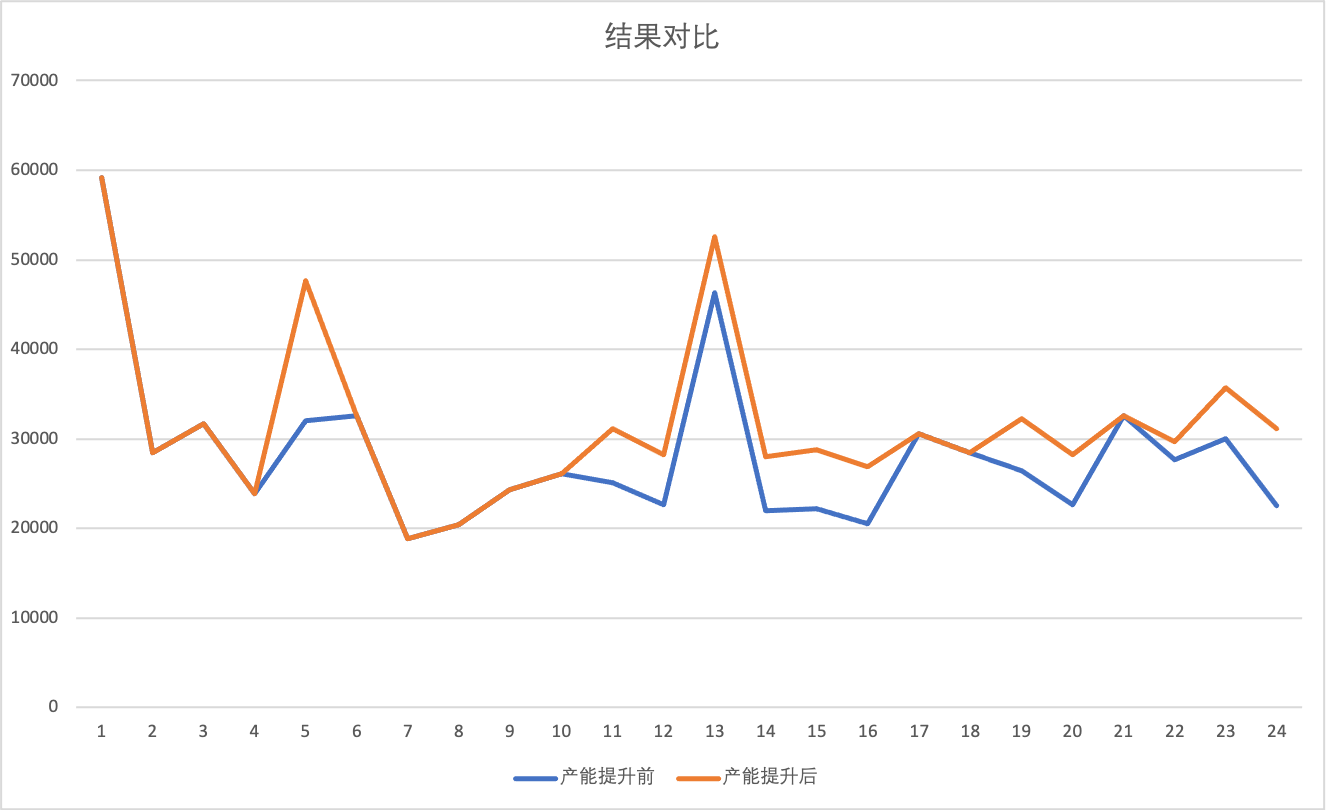
\includegraphics[width=15cm]  {产能提升对比.png}}
    \caption{订购量提升对比}
\end{figure}


%-------------------- 九、模型的分析与检验 --------------------%
\section{模型的讨论与分析}

\subsection{误差分析}
本文建立的规划模型中所用的预期供应量和损耗率都是根据历史数据算出来的固定的值,一方面本文的计算方法并不一定最科学,可能对这一数据带来一定的误差。此外,在实际情况中这两个变量都是会变化的,也会对结果带来一定的偏差。但是根据历史数据求出的指标和结果都是准确的。

\subsection{伪灵敏度分析}
本文的第二、第三、第四问问建立的模型都属于线性规划模型,而且都是整数规划问题,属于确定性算法,不存在灵敏度问题。 并且求出的方案都是全局最优解。

第一问采用主成分分析法建立评价模型,其是基于指标所用历史数据信息所占比来确定权重的,而历史数据信息是大量并且确定的,指标的数值是客观的,当历史信息准确时,灵敏度相对较好。

%-------------------- 十、模型的评价与推广 --------------------%
\section{模型的评价、改进与推广}



%----10.1 模型的优点---%
\subsection{模型的优点}


(1)评价模型考虑的指标较为全面。

(2)评价模型采用主成分分析法达到数据降维的效果,同时具有客观性。

(3)订购规划模型考虑到供货量随周期发生的变化。

(4)订购规划模型能够对24周全局进行规划,具有很好的前瞻性。

(5)订购规划模型是线性的,能够很好地被求解,且可求解到精确解。

(6)本文对每一问的求解结果都结合实际情况进行了合理性分析,保证结果的合理性。

%----10.2 模型的缺点---%
\subsection{模型的缺点}
(1)转运方案的制定假设当周的订购量等于供应量,但实际上供应量是会多于或小于订货量。

(2)本文对每周订购方案和转运方案的规划都采用了一个确定的预期供应量和损耗率,但实际情况中是会随机变化的,当变化和预期值相差大时,我们的模型不一定能够得到一个最优的方案。

(3)评价模型中对供货商时间序列的分析不够全面。

(4)规划模型中对随机性的因素考虑得较少

%----10.3 模型的改进与推广---%
\subsection{模型的推广}


本文中的评价模型可以帮助企业对众多上游供应商进行评价与选择,有利于供应链的稳定性与响应性。

本问中的规划模型在生产与运营管理中具有一定的意义,能够帮助企业进行物料资源计划的制定、生产与订购进度的安排,让企业资源计划更加具有前瞻性。


%-------------------- 参考文献 --------------------%
\begin{thebibliography}{9}%宽度9
 \bibitem{bib:one}\label{ref001} 霍佳震,雷星晖,隋明刚.基于供应链的供应商绩效评价体系研究[J].上海大学学报(自然科学版),2002(02):177-182+188.%---参考文献1---%
 \bibitem{bib:two} 司守奎, 孙玺菁. 数学建模算法与应用[M]. 国防工业出版社, 2021.%---参考文献2---%
 \bibitem{bib:three} 胡运权. 运筹学教程(第四版)[M]. 清华大学出版社, 2012.%---参考文献3---%
 \bibitem{bib:four} Hamdy A. Taha. Operations Research an Introduction[M]. Pearson Education,
 2017.%---参考文献
\end{thebibliography}



%--------------- 附录 ---------------%
\newpage
\begin{appendices}

%----支撑材料列表----%
\section{支撑材料列表}
\begin{lstlisting}[]
    code/
    supply_capacity.m 计算供应商周期内每周供货能力
    pca.m 主成分分析
    find_min_suppliers_num.py 规划最小供应商数
    order_econo_prog.py 只考虑订货成本的规划模型求解
    total_econo_prog.py 考虑综合成本的规划模型求解
    transfer_01_prog.py 基于0-1规划的转运模型求解
    transfer_int_prog.py 基于整数规划的转运模型求解
    maxify_prod.py 规划最大产能提升

    data/
    supply_capacity_avg.csv 供应商周期内每周平均供货能力
    supply_capacity_max.csv 供应商周期内每周最大供货能力
    原始指标数据.xlsx
    Q3AC.xlsx 第三问中多目标规划结果
    Q3ABC.xlsx 第三问中引入单位转运与储存成本的单目标规划结果
    Q3.xlsx 第三问中不考虑单位转运与储存成本的规划结果

    result/
    附件A 订购方案数据结果.xlsx
    附件B 转运方案数据结果.xlsx
\end{lstlisting}

%----代码1----%
\section{Matlab 源代码}
\begin{lstlisting}[language=matlab]
clc
clear

%% 计算供应商周期内每周最大供货能力
load('Q.mat')
[m, n] = size(Q);
C = [];
for r = 1:m
    R = reshape(Q(r, :), [24, 10])';
    Avg = [];
    for col = 1:24
        Col = R(:, col);
        avg = mean(maxk(Col, 2));
        Avg(end+1) = avg;
    end
    C = [C; Avg];
end

%% 计算供应商周期内每周平均供货能力
load('D.mat')
C = [];
for r = 1:m
    R1 = reshape(Q(r, :), [24, 10])';
    R2 = reshape(D(r, :), [24, 10])';
    Avg = [];
    for col = 1:24
        Col1 = R1(:, col);
        Col2 = R2(:, col);
        if sum(Col2 > 0) == 0
            avg = 0
        else
            avg = sum(Col1) / sum(Col2 > 0);
        end
        Avg(end+1) = avg;
    end
    C = [C; Avg];
end

%% 主成分分析
clear all;
table = load('原始指标数据.txt');
table = table(2:403, 2:11);
table_standard = zscore(table);
P = cov(table_standard);
[M,D] = eig(P);
d = diag(D);
S_eig = sort(d,'descend');
m = fliplr(M);
i = 0;
j = 0;
% 重要性排序后从大到小找到加和第一次超过93%所需的特征值个数
while i/sum(S_eig) < 0.93
    j = j + 1;
    i = i + S_eig(j);
end
[pc,latent,explained] = pcacov(P);
num = 5;
pc = pc.*(sign(sum(pc)));
dataframe = P * pc(:,[1:num]);
total_score = dataframe * explained(1:num)/100;
% 计算主成分得分并按照降序排列
[descend_score , number] = sort(total_score,'descend');
descend_score = descend_score';
number = number';

\end{lstlisting}

%----代码2----%
\section{Python 源代码}
\begin{lstlisting}[language=python]
    from gurobipy import *
    
    ## find_min_suppliers_num.py
    I_NUM = 402
    J_NUM = 24
    DEMAND_Q = 2.82e4
    MAX = 1e5
    MODEL = Model()
    x = MODEL.addVars(I_NUM, vtype=GRB.BINARY, name='x')
    s = MODEL.addVars(J_NUM, lb=-GRB.INFINITY, name='s')
    MODEL.update()
    MODEL.setObjective(quicksum(x[i] for i in range(I_NUM)), GRB.MINIMIZE)
    MODEL.addConstrs(quicksum(quicksum(capacity[i][j] / demand[i] * x[i] for i in range(I_NUM)) for j in range(k)) + s[k - 1] == DEMAND_Q * k for k in range(1, J_NUM + 1))
    MODEL.addConstrs(s[j] <= 0 for j in range(J_NUM))
    MODEL.optimize()

    ## order_econo_prog.py
    I_NUM = 16
    J_NUM = 24
    DEMAND_Q = 2.82e4
    MODEL = Model()
    x = MODEL.addVars(I_NUM, J_NUM, lb=0, vtype=GRB.INTEGER, name='x')
    s = MODEL.addVars(J_NUM, lb=-GRB.INFINITY, name='s')
    MODEL.update()
    MODEL.setObjective(quicksum(price[target[i] - 1] * x[i, j] for i in range(I_NUM) for j in range(J_NUM)), GRB.MINIMIZE)
    MODEL.addConstrs(quicksum(quicksum(x[i, j] / demand[target[i] - 1] for i in range(I_NUM)) for j in range(k)) + s[k - 1] >= DEMAND_Q * k for k in range(1, J_NUM + 1))
    MODEL.addConstrs(x[i, j] <= capacity[target[i] - 1][j] for i in range(I_NUM) for j in range(J_NUM))
    MODEL.addConstrs(s[j] <= 0 for j in range(J_NUM))
    MODEL.optimize()

    ## total_econo_prog.py
    I_NUM = 402
    J_NUM = 24
    DEMAND_Q = 2.82e4
    MODEL = Model()
    x = MODEL.addVars(I_NUM, J_NUM, lb=0, vtype=GRB.INTEGER, name='x')
    s = MODEL.addVars(J_NUM, lb=-GRB.INFINITY, name='s')
    MODEL.update()
    MODEL.setObjective(quicksum(price[i] * x[i, j] + weight[i] * x[i, j] for i in range(I_NUM) for j in range(J_NUM)), GRB.MINIMIZE)
    MODEL.addConstrs(quicksum(quicksum(x[i, j] / demand[i] for i in range(I_NUM)) for j in range(k)) + s[k - 1] == DEMAND_Q * k for k in range(1, J_NUM + 1))
    MODEL.addConstrs(x[i, j] <= capacity[i][j] for i in range(I_NUM) for j in range(J_NUM))
    MODEL.addConstrs(quicksum(x[i, j] for i in range(I_NUM)) <= 6000*8 for j in range(J_NUM))
    MODEL.addConstrs(s[j] <= 0 for j in range(J_NUM))
    MODEL.optimize()

    ## transfer_01_prog.py
    I_NUM = len(order_list)
    J_NUM = len(waste_rate)
    MODEL = Model()
    x = MODEL.addVars(I_NUM, J_NUM, vtype=GRB.BINARY, name='x')
    MODEL.update()
    MODEL.setObjective(quicksum(waste_rate[j] * x[i, j] * order_list[i] for i in range(I_NUM) for j in range(J_NUM)), GRB.MINIMIZE)
    MODEL.addConstrs(quicksum(x[i, j] for j in range(J_NUM)) == 1 for i in range(I_NUM))
    MODEL.addConstrs(quicksum(x[i, j] * order_list[i] for i in range(I_NUM)) <= 6e3 for j in range(J_NUM))
    MODEL.optimize()

    ## transfer_int_prog.py
    I_NUM = len(order_list)
    J_NUM = len(waste_rate)
    MODEL = Model()
    x = MODEL.addVars(I_NUM, J_NUM, lb=0, vtype=GRB.INTEGER, name='x')
    MODEL.update()
    MODEL.setObjective(quicksum(waste_rate[j] * x[i, j] for i in range(I_NUM) for j in range(J_NUM)), GRB.MINIMIZE)
    MODEL.addConstrs(quicksum(x[i, j] for j in range(J_NUM)) == order[i][week] for i in range(I_NUM))
    MODEL.addConstrs(quicksum(x[i, j] for i in range(I_NUM)) <= 6e3 for j in range(J_NUM))
    MODEL.optimize()

    ## maxify_prod.py
    I_NUM = 402
    J_NUM = 24
    MODEL = Model()
    x = MODEL.addVars(I_NUM, J_NUM, lb=0, vtype=GRB.INTEGER, name='x')
    s = MODEL.addVars(J_NUM, lb=-GRB.INFINITY, name='s')
    pm = MODEL.addVar(lb=2.82e4, ub=4.8e4, name='pm')
    MODEL.update()
    MODEL.setObjective(-pm, GRB.MINIMIZE)
    MODEL.addConstrs(quicksum(quicksum(x[i, j] / demand[i] for i in range(I_NUM)) for j in range(k)) + s[k - 1] == pm * k for k in range(1, J_NUM + 1))
    MODEL.addConstrs(x[i, j] <= capacity[i][j] for i in range(I_NUM) for j in range(J_NUM))
    MODEL.addConstrs(quicksum(x[i, j] for i in range(I_NUM)) <= 6000*8 for j in range(J_NUM))
    MODEL.addConstrs(s[j] <= 0 for j in range(J_NUM))
    MODEL.optimize()

\end{lstlisting}

\end{appendices}

\end{document} 
